\chapter{Смешивание, осцилляции, электрические дипольные моменты и полевые операторы}

Начнём немного в стороне от заявленной темы — с вопроса о нейтрино. Имеются свидетельства того, что нейтрино обладают массой и что типы нейтрино смешиваются. Если массы не у всех одинаковы, как один тип может превращаться в другой, не нарушая закон сохранения энергии?

Этот вопрос указывает на общую схему, встречающуюся повсюду в квантовой механике: состояния, в которых систему подготавливают или регистрируют, не обязаны быть состояниями, диагонализующими её гамильтониан. Состояние с определённой энергией лишь приобретает фазу. Подготовленное состояние, являющееся суперпозицией нескольких энергий, изменяется потому, что его компоненты приобретают разные фазы. Именно это различие проведёт нас от двухъямного потенциала к нейтринным осцилляциям и прецессии спина. После отступления об электрическом дипольном моменте электрона мы вернёмся ко вторичному квантованию и увидим на уровне операторов ту же координатно--импульсную фурье-структуру.

\section{Смешивание как суть вопроса}

Масса у всех нейтрино не обязана быть одинаковой. Собственные состояния энергии не смешиваются друг с другом; каждое эволюционирует независимо. То, что мы называем \emph{типом}, или ароматом, нейтрино, связано с тем, как оно рождается и регистрируется, и состояние с определённым ароматом может быть линейной комбинацией собственных состояний массы и энергии. Схематически,
\begin{equation}
|\text{type}\rangle = \sum_n c_n |E_n\rangle .
\end{equation}
Следовательно, правильно говорить не о том, что собственные состояния энергии переходят друг в друга, а о том, что состояния, называемые ``электронным нейтрино'' или ``мюонным нейтрино'', сами не обязаны быть собственными состояниями энергии.

\begin{classroomqa}
\lecturetimestamp{00:00:09}
\audiencequestion{Если массы нейтрино различны, как они могут смешиваться при сохранении энергии?}
\lecturerresponse{Собственные состояния массы и энергии не переходят друг в друга. Состояния электронного, мюонного и тау-аромата представляют собой различные линейные комбинации этих собственных состояний. Каждая массовая компонента эволюционирует со своей собственной фазой, и интерференция изменяет вероятности различных ароматов, не нарушая закона сохранения энергии.}
\end{classroomqa}

У этой структуры много примеров. Наиболее наглядный из них начинается с частицы в симметричном двухъямном потенциале.

\section{Симметричный двухъямный потенциал и приближённые локализованные состояния}

Рассмотрим частицу, движущуюся в симметричном двухъямном потенциале с высоким барьером между двумя минимумами. Если бы барьер был бесконечно высоким, левая и правая ямы были бы полностью развязаны. Можно было бы решать задачу для левой ямы так, как будто правой не существует, и аналогично для правой. Тогда приближёнными волновыми функциями основного состояния были бы локализованное слева состояние \(\psi_L\) и локализованное справа состояние \(\psi_R\), оба с одной и той же энергией \(E\).

В каждой изолированной яме основное состояние обладает привычными качественными свойствами: оно гладкое, не имеет узлов и находится при наименьшей возможной энергии, совместимой с локализацией. Представьте себе высокий центральный барьер как кирпичную стену. Рассматривать его как бесконечный — лишь приближение, но оно даёт нам полезную пару локализованных состояний, с которой можно начать.

\begin{figure}
\centering
\begin{adjustbox}{max width=\linewidth}
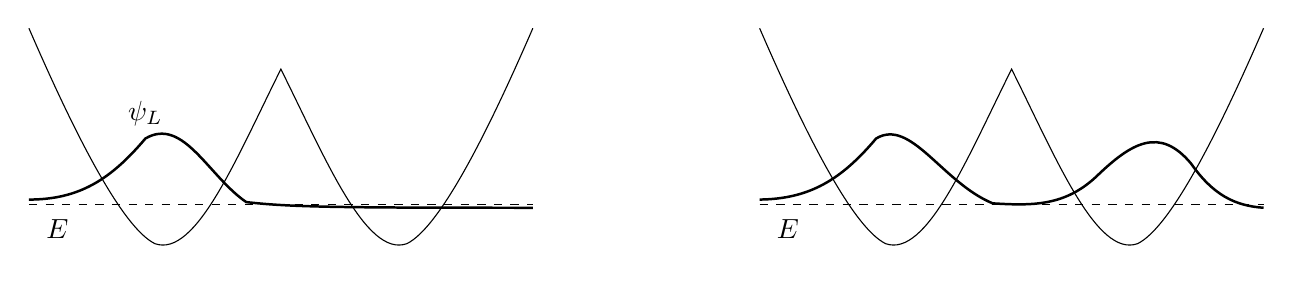
\begin{tikzpicture}[x=0.8cm,y=0.8cm]
\begin{scope}[shift={(-5.8,0)}]
\draw (-4,2.7) .. controls (-3.35,1.2) and (-2.55,-0.45) .. (-2.0,-0.72)
      .. controls (-1.35,-0.95) and (-0.7,0.65) .. (0,2.05)
      .. controls (0.7,0.65) and (1.35,-0.95) .. (2.0,-0.72)
      .. controls (2.55,-0.45) and (3.35,1.2) .. (4,2.7);
\draw[dashed] (-4,-0.10) -- (4,-0.10);
\node at (-3.55,-0.48) {$E$};
\draw[line width=0.9pt] (-4,-0.02) .. controls (-3.2,-0.02) and (-2.7,0.30) .. (-2.15,0.95)
      .. controls (-1.55,1.30) and (-1.15,0.35) .. (-0.55,-0.06)
      .. controls (0.15,-0.14) and (0.9,-0.15) .. (4,-0.15);
\node at (-2.15,1.35) {$\psi_L$};
\end{scope}
\begin{scope}[shift={(5.8,0)}]
\draw (-4,2.7) .. controls (-3.35,1.2) and (-2.55,-0.45) .. (-2.0,-0.72)
      .. controls (-1.35,-0.95) and (-0.7,0.65) .. (0,2.05)
      .. controls (0.7,0.65) and (1.35,-0.95) .. (2.0,-0.72)
      .. controls (2.55,-0.45) and (3.35,1.2) .. (4,2.7);
\draw[dashed] (-4,-0.10) -- (4,-0.10);
\node at (-3.55,-0.48) {$E$};
\draw[line width=0.9pt] (-4,-0.02) .. controls (-3.2,-0.01) and (-2.7,0.30) .. (-2.15,0.95)
      .. controls (-1.6,1.28) and (-1.1,0.25) .. (-0.30,-0.08)
      .. controls (0.35,-0.12) and (0.85,-0.12) .. (1.35,0.35)
      .. controls (1.9,0.88) and (2.35,1.15) .. (2.85,0.55)
      .. controls (3.2,0.05) and (3.55,-0.12) .. (4,-0.15);
\end{scope}
\end{tikzpicture}
\end{adjustbox}
\caption{Аккуратно перерисованный набросок с начальной доски. Слева показано одностороннее пробное состояние \(\psi_L\), полученное при предположении, что барьер фактически бесконечен. Справа та же волновая функция симметрично продолжена через барьер, что иллюстрирует малую, но ненулевую утечку, которая в конечном счёте приводит к истинному чётному основному состоянию.}
\end{figure}

С точки зрения квантовой механики, однако, барьер не является по-настоящему бесконечным. Волновая функция в области барьера не обращается точно в нуль; она лишь очень мала. Вся суть — в этой крошечной утечке. Именно она превращает лево-правое приближение в подлинную задачу о смешивании.

\section{Собственные состояния чётности и экспоненциальное расщепление уровней}

Теперь в эту локализованную картину вмешивается теорема: если потенциал симметричен, то точные собственные функции энергии можно выбрать либо симметричными, либо антисимметричными относительно отражения.

\begin{theorem}
Если \(V(x)=V(-x)\) в одном измерении, то собственные функции гамильтониана можно выбрать так, чтобы они удовлетворяли либо
\[
\psi(x)=\psi(-x)
\qquad \text{or} \qquad
\psi(x)=-\psi(-x).
\]
\end{theorem}

Теперь нужно внести поправку. Односторонние состояния \(\psi_L\) и \(\psi_R\) не являются ни симметричными, ни антисимметричными, поэтому они не могут быть точными собственными состояниями полного гамильтониана. Они являются хорошими приближёнными состояниями лишь тогда, когда барьер высок. Истинные собственные состояния — симметричная и антисимметричная комбинации,
\begin{align}
\psi_+ &= \frac{\psi_L+\psi_R}{\sqrt{2}},\\
\psi_- &= \frac{\psi_L-\psi_R}{\sqrt{2}}.
\end{align}
В обозначениях, которые и дальше останутся на доске, обозначим их энергии как
\begin{align}
H\psi_+ &= (E_1-\epsilon)\psi_+,\\
H\psi_- &= (E_1+\epsilon)\psi_-.
\end{align}
Тогда полное расщепление равно
\begin{equation}
\Delta E = (E_1+\epsilon)-(E_1-\epsilon)=2\epsilon .
\end{equation}

\begin{figure}[htbp]
\centering
\includegraphics[width=0.92\linewidth]{lecture_08_frame_02.png}
\caption{Волновая функция, симметрично продолженная в двухъямном потенциале. Её амплитуда под барьером мала, но не равна нулю, и именно это служит источником расщепления уровней.}
\lectureframe{00:06:19}
\end{figure}

\begin{figure}
\centering
\begin{tikzpicture}[x=1cm,y=1cm]
\draw[->] (0,0) -- (0,3);
\node[left] at (0,2.8) {energy};
\draw (-0.35,1.60) -- (0.35,1.60);
\node[left] at (-0.45,1.60) {$\psi_L,\psi_R$};
\node at (1.7,1.60) {$\Longrightarrow$};
\draw (3.0,1.32) -- (3.75,1.32);
\draw (3.0,1.88) -- (3.75,1.88);
\draw[dashed] (2.8,1.60) -- (3.95,1.60);
\node[right] at (3.9,1.32) {$\psi_+,\ E_1-\epsilon$};
\node[right] at (3.9,1.88) {$\psi_-,\ E_1+\epsilon$};
\node[below] at (3.37,1.60) {$E_1$};
\end{tikzpicture}
\caption{Логика туннельного расщепления, показанная на доске. Приближённые левые и правые состояния почти вырождены, но точные симметричное и антисимметричное собственные состояния расщеплены на малую величину \(2\epsilon\).}
\end{figure}

Упорядочение уровней и несёт физический смысл. Симметричное состояние имеет чуть меньшую энергию, потому что оно более гладко проходит через область барьера; то, что волновой функции позволено просачиваться и симметрично продолжаться, понижает энергию на крошечную величину. Антисимметричное состояние имеет чуть большую энергию, потому что первое возбуждённое состояние в одном измерении имеет один узел, и в этой симметричной задаче этот узел расположен в середине. Дополнительная кривизна увеличивает кинетическую энергию.

Эффект очень мал — экспоненциально мал по ширине и высоте барьера. Явная формула WKB нам здесь не нужна; важно, что расщепление реально, но мало. Помните также, что общий знак волновой функции не несёт физической информации. Замена \(\psi_-\) на \(-\psi_-\) не изменяет состояния.

\section{Эволюция во времени и лево-правые осцилляции}

Теперь зададим динамический вопрос: что происходит, если мы помещаем частицу в левую яму? Это решающий шаг, потому что осцилляция — это зависящее от времени проявление того же самого явления смешивания.

Обратные соотношения имеют вид
\begin{align}
\psi_L &= \frac{\psi_+ + \psi_-}{\sqrt{2}},\\
\psi_R &= \frac{\psi_+ - \psi_-}{\sqrt{2}}.
\end{align}
Поэтому первоначально локализованное слева состояние равно
\begin{equation}
\psi(0)=\psi_L=\frac{\psi_+ + \psi_-}{\sqrt{2}}.
\end{equation}
Это не собственное состояние энергии, и потому оно должно эволюционировать нетривиально.

Мы используем стандартное Schr\"odinger-соглашение \(e^{-iEt}\). Общая фаза не оказывает наблюдаемого эффекта; лишь относительная фаза между двумя энергетическими компонентами может переносить вероятность из одной ямы в другую.

С этим соглашением,
\begin{equation}
\psi(t)=\frac{1}{\sqrt{2}}\left(e^{-i(E_1-\epsilon)t}\psi_+ + e^{-i(E_1+\epsilon)t}\psi_-\right).
\end{equation}
Это приведённая в порядок версия формулы с доски. Теперь вынесем общую фазу:
\begin{equation}
\psi(t)=\frac{e^{-iE_1 t}}{\sqrt{2}}\left(e^{i\epsilon t}\psi_+ + e^{-i\epsilon t}\psi_-\right).
\end{equation}
Теперь одна фаза обходит единичную окружность в одну сторону, а другая — в противоположную. Состояние изменяется только потому, что эти две фазы постепенно расходятся по фазе.

Чтобы явно увидеть лево-правые осцилляции, подставим определения \(\psi_\pm\):
\begin{align}
\psi(t)
&= \frac{e^{-iE_1 t}}{2}
\left[e^{i\epsilon t}(\psi_L+\psi_R)+e^{-i\epsilon t}(\psi_L-\psi_R)\right] \\
&= \frac{e^{-iE_1 t}}{2}
\left[(e^{i\epsilon t}+e^{-i\epsilon t})\psi_L+(e^{i\epsilon t}-e^{-i\epsilon t})\psi_R\right] \\
&= e^{-iE_1 t}\left[\psi_L\cos(\epsilon t)+i\,\psi_R\sin(\epsilon t)\right].
\end{align}
Это ключевой подробно разобранный вывод этой главы. В двухсостояниевом приближении, где \(\psi_L\) и \(\psi_R\) ортонормированы, вероятности равны
\begin{equation}
P_L(t)=\cos^2(\epsilon t),
\qquad
P_R(t)=\sin^2(\epsilon t).
\end{equation}
Итак, система осциллирует. В промежуточные моменты времени она действительно находится в суперпозиции; например, при \(\epsilon t=\pi/4\) вероятности по обе стороны одинаковы. Фазы эволюционируют непрерывно, и локализация меняется непрерывно вместе с ними.

Вывод на доске выделяет первый момент времени, в который относительный знак меняется. Спрашивается, когда
\begin{equation}
e^{-i\epsilon t}=-\,e^{i\epsilon t},
\end{equation}
что и является заметной вехой на доске. После умножения получаем
\begin{equation}
e^{2i\epsilon t}=-1.
\end{equation}
При первом таком случае,
\begin{equation}
2\epsilon t=\pi,
\qquad\text{so}\qquad
t_{L\to R}=\frac{\pi}{2\epsilon}.
\end{equation}

\begin{figure}[htbp]
\centering
\includegraphics[width=0.94\linewidth]{lecture_08_frame_05.png}
\caption{Вычисление относительной фазы на доске. Две энергетические компоненты становятся противоположными при \(e^{2i\epsilon t}=-1\), что даёт первое время перехода \(2\epsilon t=\pi\). В набранном выводе используется одно последовательное Schr\"odinger-фазовое соглашение.}
\lectureframe{00:17:52}
\end{figure}
В этот момент,
\begin{equation}
\psi(t_{L\to R}) \propto \frac{\psi_+-\psi_-}{\sqrt{2}}=\psi_R.
\end{equation}
Общая фаза несущественна. Важно то, что частица, первоначально помещённая слева, эволюционировала в локализованное справа состояние. Ещё через такой же интервал она снова вернётся назад. Смешивание и осцилляция идут вместе.

Уравнение однозначно: малое \(\epsilon\) означает медленные осцилляции и длительное время перехода. Ни одно из локализованных состояний не имеет определённой энергии, но обе точные энергетические компоненты сохраняют энергию и эволюционируют в точности так, как должны.

\section{Аналогии с нейтрино, аммиаком и спином}

Двухъямный потенциал даёт нам схему для исходного вопроса о нейтрино. Нейтрино, рождённое вместе с электроном, называется электронным нейтрино; рождённое вместе с мюоном — мюонным нейтрино. Эти ароматовые метки описывают каналы рождения и регистрации. Состояния с определёнными массами и, следовательно, при фиксированном импульсе с определёнными энергиями свободной частицы образуют другой базис.

В простейшей схематичной двухсостоянийной модели с максимальным смешиванием,
\begin{equation}
|\nu_e\rangle \sim \frac{|m_1\rangle+|m_2\rangle}{\sqrt{2}},
\qquad
|\nu_\mu\rangle \sim \frac{|m_1\rangle-|m_2\rangle}{\sqrt{2}},
\end{equation}
где массовые собственные состояния играют роль \(\psi_+\) и \(\psi_-\), а состояния аромата играют роль \(\psi_L\) и \(\psi_R\). В реальном смешивании нейтрино вместо этих равных коэффициентов используется нетривиальная матрица смешивания, но сам механизм уже виден и здесь.

Нейтрино электронного аромата рождается в процессе с участием электрона, подобно тому как частицу можно поместить в левую яму. За короткое время распространения две его массовые компоненты накапливают почти одинаковую фазу, так что взаимодействие всё ещё идентифицирует его как нейтрино электронного аромата. На длинной базе их фазы расходятся. Тогда более позднее взаимодействие по заряженному току может породить мюон, а не электрон: состояние приобрело компоненту мюонного аромата. Повторяя эксперимент при разных расстояниях или энергиях, можно обнаружить осцилляцию.

Никакого конфликта с сохранением энергии здесь нет. Собственные состояния массы-энергии делают в точности то, что и должны делать собственные состояния. Эволюционирует именно суперпозиция по аромату. В релятивистском пределе наблюдаемая относительная фаза определяется разностями квадратов масс, схематически
\begin{equation}
\Delta\phi_{ij}\simeq \frac{\Delta m_{ij}^{,2}L}{2E}.
\end{equation}
Следовательно, осцилляция показывает, что не все массы нейтрино могут быть одинаковыми; по меньшей мере два массовых собственных состояния различаются по массе.

\begin{classroomqa}
\lecturetimestamp{00:24:06}
\audiencequestion{От чего зависит малое расщепление \(\epsilon\) в примере с двойной ямой?}
\lecturerresponse{Оно зависит от массы частицы, а также от высоты и ширины барьера. Туннелирование экспоненциально чувствительно к этим деталям, поэтому умеренное изменение барьера может вызвать большое относительное изменение \(\epsilon\).}
\end{classroomqa}

\begin{classroomqa}
\lecturetimestamp{00:24:26}
\audiencequestion{Наблюдалось ли это явление осцилляции в действительности?}
\lecturerresponse{Да. Туннельные расщепления наблюдаются в обычных квантовых системах, а осцилляции аромата наблюдаются у нейтрино. Микроскопические механизмы различаются, но в обоих случаях реализуется одна и та же двухсостоянийная фазовая эволюция.}
\end{classroomqa}

\begin{classroomqa}
\lecturetimestamp{00:24:34}
\audiencequestion{Как связана осцилляция нейтрино с массой нейтрино?}
\lecturerresponse{Распространяющиеся собственные состояния имеют разные массы и потому накапливают разные фазы. Их интерференция меняет состав по аромату. В реалистическом релятивистском описании осцилляцию определяют разности квадратов масс, а не буквально изменяющаяся со временем масса одной частицы.}
\end{classroomqa}

\begin{classroomqa}
\lecturetimestamp{00:25:02}
\audiencequestion{Масса нейтрино — это лишь преобладающая теория, или это экспериментальный факт?}
\lecturerresponse{Осцилляция — экспериментальный факт, и она требует ненулевых разностей масс. Абсолютный масштаб масс — отдельное и более трудное измерение, но минимальная картина, в которой все нейтрино безмассовы, экспериментально исключена.}
\end{classroomqa}

\subsection{Инверсия аммиака: буквальный барьер}

Молекула аммиака, \(\mathrm{NH}_3\), имеет тригонально-пирамидальную форму: три атома водорода образуют плоскость, а атом азота находится по одну сторону от неё. Существует эквивалентная конфигурация, в которой атом азота расположен по другую сторону. Эти две локализованные конфигурации не являются точными стационарными состояниями. Атом азота может туннелировать через плоскость атомов водорода, образуя симметричное и антисимметричное энергетические собственные состояния и малое инверсионное расщепление. Это и есть физический источник той же математики в аммиачном мазере.

\begin{classroomqa}
\lecturetimestamp{00:25:11}
\audiencequestion{В аммиаке барьером является конфигурация, в которой азот проходит через плоскость водородов?}
\lecturerresponse{Да. Энергия молекулы минимальна в каждой из двух пирамидальных конфигураций, тогда как плоская конфигурация лежит выше. Туннелирование через эту конфигурацию связывает две стороны.}
\end{classroomqa}

\begin{classroomqa}
\lecturetimestamp{00:27:10}
\audiencequestion{Каков соответствующий физический барьер между электронным и мюонным нейтрино?}
\lecturerresponse{Буквального пространственного барьера нет. Аналогия алгебраическая: недиагональная связь в гамильтониане нейтрино смешивает базис состояний аромата. В аммиаке эта связь возникает из-за туннелирования; для нейтрино она является частью структуры масс и смешивания.}
\end{classroomqa}

\subsection{Прецессия спина: смешивание без туннелирования}

С той же алгеброй мы уже встречались для спина. Рассмотрим два состояния \(|\uparrow_z\rangle\) и \(|\downarrow_z\rangle\). В отсутствие магнитного поля они вырождены. Теперь включим магнитное поле в направлении \(x\). Энергетические собственные состояния теперь уже не совпадают с собственными состояниями \(z\), а являются состояниями, поляризованными вдоль \(x\). Пользуясь временными обозначениями левый--правый, введёнными на доске,
\begin{align}
|L_x\rangle &= \frac{|\uparrow_z\rangle+|\downarrow_z\rangle}{\sqrt{2}},\\
|R_x\rangle &= \frac{|\uparrow_z\rangle-|\downarrow_z\rangle}{\sqrt{2}}.
\end{align}
Это прямые аналоги \(\psi_+\) и \(\psi_-\). Для магнитного момента, сонаправленного и противонаправленного полю, энергии слегка различаются. Если эти энергии равны \(E\mp\epsilon\), то спин, изначально направленный вверх, эволюционирует как
\begin{equation}
|\uparrow_z,t\rangle
= e^{-iEt}\left[\cos(\epsilon t)\,|\uparrow_z\rangle
+ i\sin(\epsilon t)\,|\downarrow_z\rangle\right].
\end{equation}
Это та же формула, что и для двойной ямы, только теперь непрерывная эволюция представляет собой прецессию спина вокруг оси \(x\). Начиная с \(+z\), спин проходит через поперечные направления, достигает \(-z\) через половину периода прецессии и возвращается ещё через половину периода. Измерение \(S_z\) по-прежнему даёт только вверх или вниз; непрерывно меняющееся спиновое состояние определяет их вероятности. Этот механизм не требует туннелирования. Требуется лишь, чтобы гамильтониан был диагонален в базисе, отличном от базиса, в котором состояние приготовлено.

\begin{classroomqa}
\lecturetimestamp{00:32:25}
\audiencequestion{Что происходит в этой картине с тау-нейтрино?}
\lecturerresponse{Оно тоже смешивается. В реальной задаче есть три состояния аромата и три массовых состояния, поэтому двухсостоянийный поворот заменяется матрицей смешивания размера три на три. Сам принцип фазовой интерференции не меняется.}
\end{classroomqa}

\begin{classroomqa}
\lecturetimestamp{00:32:57}
\audiencequestion{Сразу после включения поперечного поля остаётся ли спин направленным вверх и может ли он быть направлен к нам или от нас?}
\lecturerresponse{Через очень малое время вероятность направления вверх всё ещё почти равна единице, а вероятность вниз мала. Состояние непрерывно прецессирует вокруг оси поля и проходит через поперечные направления \(\pm y\), оставаясь перпендикулярным полю, направленному вдоль \(x\), если оно начинало перпендикулярно ему. Измерение вдоль любой выбранной оси всё равно даёт одно из дискретных собственных значений этой оси.}
\end{classroomqa}

\begin{classroomqa}
\lecturetimestamp{00:34:30}
\audiencequestion{Поле выбирают слабым, чтобы спин никогда не указывал вдоль поля?}
\lecturerresponse{Нет. Геометрия определяется прецессией вокруг оси поля, а не слабостью самого поля. Слабое поле лишь делает энергетическое расщепление и частоту прецессии малыми, задавая медленную осцилляцию, аналогичную примеру с нейтрино.}
\end{classroomqa}

Величина нейтринного смешивания и малые массы нейтрино являются параметрами, более глубокое происхождение которых не объясняется минимальной Стандартной моделью в её исходной формулировке. Поэтому масса нейтрино указывает за пределы этой минимальной модели, хотя наблюдаемая шкала очень мала и может отражать физику на весьма далёкой энергетической шкале.

\begin{classroomqa}
\lecturetimestamp{00:36:27}
\audiencequestion{Является ли осцилляция причиной, по которой мы знаем, что у нейтрино есть масса?}
\lecturerresponse{Это решающее прямое свидетельство того, что распространяющиеся компоненты имеют разные массы. Если бы все соответствующие компоненты были точно безмассовыми и вырожденными, они не накапливали бы зависящей от массы относительной фазы, и вакуумной осцилляции аромата такого рода не было бы.}
\end{classroomqa}

\begin{classroomqa}
\lecturetimestamp{00:37:57}
\audiencequestion{Через полпериода должно ли нейтрино вести себя наполовину как нейтрино электронного аромата и наполовину как нейтрино мюонного аромата?}
\lecturerresponse{В идеальной симметричной двухсостоянийной модели равные вероятности возникают через четверть полного периода вероятности, тогда как полное превращение происходит при первом максимуме. Реальные трёхароматные осцилляции имеют неравные углы смешивания, несколько частот, спин-гелицитные ограничения и эффекты вещества, так что полное симметричное превращение не является типичным.}
\end{classroomqa}

\begin{classroomqa}
\lecturetimestamp{00:38:36}
\audiencequestion{Если массовые компоненты различаются, должна ли скорость солнечного нейтрино изменяться для сохранения импульса?}
\lecturerresponse{Состояние аромата представляет собой когерентную суперпозицию компонент с фиксированными массами; его масса не является классической величиной, осциллирующей во времени. В обычном описании с равными импульсами компоненты имеют слегка разные энергии и групповые скорости, тогда как в описании с равными энергиями у них слегка разные импульсы. При последовательном рассмотрении обе конвенции дают одну и ту же наблюдаемую фазу осцилляции.}
\end{classroomqa}

Эта фазовая эволюция разрешила старую проблему дефицита солнечных нейтрино. Первые детекторы были в основном чувствительны к нейтрино электронного аромата, поэтому нейтрино, покинувшие Солнце в электронном аромате, могли приходить частично в мюонном или тау-аромате и ускользать от регистрации в этом канале. Детальный расчёт для Солнца включает трёхароматное смешивание и эффекты вещества, но концептуальный урок уже содержится в двойной яме: приготовление и распространение используют разные базисы.

\section{Отступление: электрический дипольный момент, симметрия и утверждение ``электрон — сфера''}

Раз уж речь уже зашла о феноменологии частиц, отвлечёмся ненадолго от формальной математики. В популярной статье новое ограничение на электрический дипольный момент электрона было изложено так, будто показано, что электрон — сфера. Этот лозунг смешивает три разных вопроса: что измеряет электрический дипольный момент, что означает вращательная симметрия для квантового состояния и что эксперимент в действительности ограничил.

\subsection{Что было измерено?}

То, что измеряли, или, точнее, на что устанавливали ограничение, — это электрический дипольный момент электрона. Для разнесённых зарядов \(\pm q\) дипольный момент равен
\begin{equation}
\mathbf d = q\,\boldsymbol{\ell},
\end{equation}
где \(\boldsymbol{\ell}\) — вектор разделения. Ненулевой дипольный момент означает, что распределение заряда смещено относительно некоторого центра.

Для электрона, однако, существенный вопрос состоит не просто в том, смещён ли заряд от центра в каком-то произвольном направлении. У электрона есть спин и, следовательно, ось. У него также есть магнитный момент. Физически осмысленный вопрос состоит в том, существует ли корреляция между смещением заряда и этой осью:
\begin{equation}
\mathbf d_e \parallel \boldsymbol{\mu}_e
\qquad \text{or equivalently} \qquad
\mathbf d_e \parallel \mathbf S .
\end{equation}
Именно эта корреляция и имеется в виду под электрическим дипольным моментом электрона. На понятийном уровне спрашивают, приводит ли помещение спин-поляризованного электрона в электрическое поле к расщеплению двух ориентаций спина:
\begin{equation}
H_{\mathrm{EDM}}=-\mathbf d_e\cdot \mathbf E,
\qquad
\mathbf d_e=d_e\frac{\mathbf S}{|\mathbf S|}.
\end{equation}
Реальный лабораторный эксперимент гораздо тоньше, чем просто голый электрон между пластинами конденсатора, но он использует именно эту идею симметрии и сдвига энергии.

\subsection{Почему отсутствие электрического дипольного момента не означает сферичности}

Первое уточнение элементарно. Тело может не иметь дипольного момента и всё же не быть сферическим. Центрированный эллипсоид имеет по одну сторону столько же заряда, сколько и по другую, и потому не имеет диполя, хотя может иметь квадрупольный момент. Ещё более сложное распределение может не иметь ни диполя, ни квадруполя, сохраняя при этом более высокий мультипольный момент. Измерение одного мультипольного коэффициента не определяет форму целиком.

В квантовой механике слово ``форма'' требует большей осторожности. Представьте себе двухатомную, гантелеобразную молекулу с приблизительно фиксированной длиной связи. Пренебрежём радиальными колебаниями и оставим только вращения. Её вращательные состояния характеризуются угловым моментом. Если молекула бозонная, её низшее вращательное состояние имеет \(J=0\). Поскольку угловой момент порождает вращения,
\begin{equation}
\begin{gathered}
J=0 \quad\Longrightarrow\\
\text{rotationally invariant ground state.}
\end{gathered}
\end{equation}
Квантовое состояние инвариантно относительно вращений, хотя всякая картина с определённой ориентацией выглядит как гантель. Его можно описать как когерентную суперпозицию всех ориентаций. Называть это состояние ``сферическим'' полезно для одних измерений и вводит в заблуждение для других.

Сделаем мгновенный снимок. Такой снимок является измерением ориентации, и достаточно точное измерение ориентации оставляет систему в состоянии, локализованном по углу. Такое состояние не может одновременно иметь определённый угловой момент. Это вращательный вариант принципа неопределённости координата--импульс: локализация угла неизбежно вносит разброс по угловым моментам и, следовательно, вращательное возбуждение.

Для жёсткого ротора
\begin{equation}
E_J=\frac{J(J+1)}{2I},
\end{equation}
так что энергия, необходимая для разрешения структуры, определяется моментом инерции \(I\). У гантели из спортивного зала \(I\) огромен, и её вращательные уровни фантастически близки; обычный свет легко может возмутить её настолько, чтобы выявить ориентацию. У молекулы расстояние между уровнями больше. У компактного адрона оно ещё гораздо больше. Если у зонда недостаточно энергии, чтобы возбудить первую различимую вращательную структуру, повторные измерения видят лишь вращательно усреднённое основное состояние.

Мезон можно грубо представлять как двухчастичную систему кварк--антикварк. Его первые орбитальные возбуждения стоят сотни миллионов электрон-вольт и более, что намного превышает энергию оптического фотона. Поэтому низкоэнергетический зонд не может сделать мгновенный снимок внутренней ориентации. ``Сфера или нет'' — это отчасти вопрос о том, какое состояние приготовлено, а отчасти — вопрос о разрешении прибора.

Электрон делает этот вопрос более острым. Это частица со спином \(\tfrac12\), а не вращательный скаляр. Спин-поляризованное состояние задаёт ось и магнитный момент. Привычная картина циркуляции заряда вокруг этой оси — лишь эвристика---точечная дираковская частица не является буквально крошечным вращающимся шариком---но она правильно напоминает нам, что магнитный момент меняет знак вместе со спином. Вопрос об электрическом дипольном моменте состоит в том, коррелирует ли смещение электрического заряда с той же осью. Нулевой результат не превращает электрон в классическую сферу.

\begin{classroomqa}
\lecturetimestamp{00:57:30}
\audiencequestion{Не нарушило бы смещение части заряда электрона квантование заряда?}
\lecturerresponse{Нет. Квантование заряда фиксирует полный заряд. Дипольный момент относится к первому пространственному моменту этого распределения заряда или, эквивалентно, к допустимому для точечной частицы взаимодействию с электрическим полем; он не требует дробного изменения полного заряда.}
\end{classroomqa}

\begin{classroomqa}
\lecturetimestamp{00:58:00}
\audiencequestion{Запрещены ли электрические дипольные моменты квантовой теорией поля?}
\lecturerresponse{Не самой квантовой теорией поля. Они запрещены, если точны определённые дискретные симметрии. Как только эти симметрии нарушаются, оператор электрического дипольного момента становится разрешённым, хотя его коэффициент может быть чрезвычайно мал.}
\end{classroomqa}

\subsection{Чётность и обращение времени}

Подлинное содержание обсуждения электрического дипольного момента — симметрия. При преобразовании чётности электрический дипольный момент преобразуется как обычный полярный вектор, тогда как магнитный момент — как аксиальный вектор:
\begin{align}
P:\qquad &\mathbf d_e \to -\mathbf d_e,
&\boldsymbol{\mu}_e \to \boldsymbol{\mu}_e .
\end{align}
При обращении времени циркулирующий ток, определяющий магнитный момент, обращается, а статическое электрическое смещение — нет:
\begin{align}
T:\qquad &\mathbf d_e \to \mathbf d_e,
&\boldsymbol{\mu}_e \to -\boldsymbol{\mu}_e .
\end{align}
Следовательно, ненулевой электрический дипольный момент, ориентированный вдоль оси спина электрона, запрещён как точной симметрией чётности, так и точной симметрией обращения времени:
\begin{equation}
(P\ \text{exact}) \Rightarrow \mathbf d_e=0,
\qquad
(T\ \text{exact}) \Rightarrow \mathbf d_e=0.
\end{equation}

Геометрию стоит расписать подробнее. Магнитный момент создаётся током, текущим по петле. Зеркальное отражение меняет знак обычных полярных векторов, но оставляет аксиальный вектор, нормальный к этой петле, неизменным. Смещение заряда вдоль оси, напротив, меняет знак. Поэтому электрон, для которого \(\mathbf d_e\) параллелен \(\boldsymbol\mu_e\), при зеркальном отражении перешёл бы в электрон с той же магнитной ориентацией, но с противоположным соотношением между электрическим и магнитным моментами. Если бы чётность была точной и существовал лишь один вид электрона, эти два описания должны были бы представлять одну и ту же частицу; согласуется только \(d_e=0\).

Обращение времени приводит к тому же выводу иным способом. При прокрутке плёнки назад ток обращается и, следовательно, \(\boldsymbol\mu_e\) меняет знак, но статическое смещение заряда при этом не меняется. Состояние с параллельными моментами переходит в состояние с антипараллельными моментами. Точная симметрия обращения времени снова потребовала бы \(d_e=0\).

\begin{figure}[htbp]
\centering
\begin{tikzpicture}[>=Stealth,scale=0.95]
  \node[font=\bfseries] at (1.0,2.25) {original};
  \draw[->,very thick,blue!70!black] (0.65,0) -- (0.65,1.65);
  \draw[->,very thick,red!75!black] (1.35,0) -- (1.35,1.65);
  \node[blue!70!black,below] at (0.65,0) {$\boldsymbol\mu$};
  \node[red!75!black,below] at (1.35,0) {$\mathbf d$};

  \node[font=\bfseries] at (4.5,2.25) {parity};
  \draw[->,very thick,blue!70!black] (4.15,0) -- (4.15,1.65);
  \draw[->,very thick,red!75!black] (4.85,1.65) -- (4.85,0);
  \node[blue!70!black,below] at (4.15,0) {$\boldsymbol\mu$};
  \node[red!75!black,below] at (4.85,0) {$-\mathbf d$};

  \node[font=\bfseries] at (8.0,2.25) {time reversal};
  \draw[->,very thick,blue!70!black] (7.65,1.65) -- (7.65,0);
  \draw[->,very thick,red!75!black] (8.35,0) -- (8.35,1.65);
  \node[blue!70!black,below] at (7.65,0) {$-\boldsymbol\mu$};
  \node[red!75!black,below] at (8.35,0) {$\mathbf d$};
\end{tikzpicture}
\caption{Проверка симметрий, восстановленная по аргументу на доске. Чётность обращает электрический диполь, но не аксиальный магнитный момент; обращение времени обращает магнитный момент, но не статическое электрическое смещение. Каждая из этих точных симметрий по отдельности запрещает постоянный электрический дипольный момент, параллельный спину.}
\end{figure}

\begin{figure}[htbp]
\centering
\includegraphics[width=0.94\linewidth]{lecture_08_frame_06.png}
\caption{Парные наброски магнитной оси и смещения заряда в ходе рассуждения об обращении времени. Компактная диаграмма TikZ выше отделяет содержание преобразования от частично стёртой доски на лекции.}
\lectureframe{01:06:10}
\end{figure}

\begin{classroomqa}
\lecturetimestamp{01:06:38}
\audiencequestion{При обращении времени обращаются ли и токи, и заряды?}
\lecturerresponse{Токи обращаются, потому что обращаются скорости; сам электрический заряд — нет. Знак заряда меняет зарядовое сопряжение \(C\), а не обращение времени \(T\).}
\end{classroomqa}

\begin{classroomqa}
\lecturetimestamp{01:07:01}
\audiencequestion{Означает ли антиунитарный характер обращения времени, что нерелятивистская квантовая механика не инвариантна относительно обращения времени?}
\lecturerresponse{Нет. Антиунитарность — это как раз тот способ, которым обращение времени согласованно реализуется в квантовой механике: оно комплексно сопрягает амплитуды и обращает импульсы и спины. Инвариантен ли конкретный гамильтониан — отдельный вопрос.}
\end{classroomqa}

\begin{classroomqa}
\lecturetimestamp{01:07:19}
\audiencequestion{Требует ли обсуждение электрического дипольного момента, чтобы электрон имел конечный объём, а не был точечным?}
\lecturerresponse{Нет. Эффективный гамильтониан точечной частицы может содержать \(-d_e\,\widehat{\mathbf S}\!\cdot\!\mathbf E\). Эксперимент спрашивает, приобретают ли противоположные ориентации спина разные энергии в электрическом поле; ему не требуется разрешать буквальное протяжённое облако заряда.}
\end{classroomqa}

Чётность не является симметрией слабых взаимодействий; в их хиральных связях она нарушается максимально сильно. Обращение времени тоже не является точной симметрией, но известное нарушение в Стандартной модели даёт вклад в ЭДМ электрона лишь на чрезвычайно малом уровне. Можно вычислить ненулевой вклад Стандартной модели, однако он лежит намного ниже чувствительности, о которой здесь идёт речь. Поэтому нулевой результат согласуется со Стандартной моделью, одновременно сужая пространство для её расширений---например, суперсимметрии и других новых взаимодействий---которые могут порождать гораздо более сильное нарушение обращения времени.

Основная экспериментальная идея проста. Магнитное поле выявляет магнитный диполь, расщепляя спиновые ориентации. Электрическое поле выявило бы ЭДМ по дополнительному сдвигу энергии, коррелированному со спином. В реальных прецизионных экспериментах используют атомы или молекулы, длительные времена когерентной прецессии, обращения приложенных полей и тщательный контроль систематических эффектов, а не изолированный электрон в наивной установке.

\begin{classroomqa}
\lecturetimestamp{01:11:02}
\audiencequestion{Был ли поиск ЭДМ экспериментом по столкновениям при высоких энергиях или экспериментом с материальными объектами?}
\lecturerresponse{Это был прецизионный настольный эксперимент: использовались электроны, связанные в контролируемой атомной или молекулярной среде, вместе с электрическими и магнитными полями. Энергия в нём низка, но чувствительность к крошечным сдвигам, нарушающим симметрии, косвенно зондирует новую физику высоких энергий.}
\end{classroomqa}

\begin{classroomqa}
\lecturetimestamp{01:12:21}
\audiencequestion{Накладывает ли нулевой результат ограничения на то, какие модификации Стандартной модели остаются жизнеспособными?}
\lecturerresponse{Да, в принципе: каждая модель предсказывает некоторый коэффициент и тем самым соответствует некоторой области параметров. Детальное численное исключение требует специального расчёта, но общая логика надёжна---более точное согласие со Стандартной моделью оставляет меньше места для альтернатив, предсказывающих большой ЭДМ.}
\end{classroomqa}

\begin{classroomqa}
\lecturetimestamp{01:13:09}
\audiencequestion{Требуется ли симметрия обращения времени для сохранения квантовой информации?}
\lecturerresponse{Нет. Унитарная эволюция во времени сохраняет информацию, даже когда гамильтониан не инвариантен относительно \(T\). Частица в фиксированном магнитном поле — привычный пример: в фильме, прокрученном назад во времени, поле выделяет определённую ориентацию, если только не обратить и само поле, и всё же квантовая эволюция остаётся унитарной. При обычных предположениях локальной лоренц-инвариантной квантовой теории поля совместное преобразование \(CPT\) является симметрией, но унитарность гарантируется не этим.}
\end{classroomqa}

Теперь перерыв можно завершить. Нулевой результат измерения говорит, что при заявленной чувствительности у электрона не обнаружено ЭДМ. Он не говорит, что электрон является сферой, и не опровергает Стандартную модель; он затрудняет обоснование некоторых предложенных отклонений от этой модели.

\section{Возвращение ко вторичному квантованию: преобразования Фурье, импульсные моды и локальность}

Мы занимались вторичным квантованием. Давайте аккуратно начнём сначала: с хорошо знакомого факта об обычных одночастичных волновых функциях, а затем перенесём его на операторы. Связь с преобразованиями Фурье здесь точна и проста.

\subsection{От координатного пространства к импульсному пространству}

Волновая функция одной частицы — это строчная \(\psi\), а не заглавная \(\Psi\). В координатном пространстве,
\begin{equation}
P(x)=|\psi(x)|^2
\end{equation}
есть плотность вероятности найти частицу в положении \(x\). Волновая функция в импульсном пространстве получается из неё преобразованием Фурье,
\begin{equation}
\tilde{\psi}(p)=\int dx\,\psi(x)\,\frac{e^{-ipx}}{\sqrt{2\pi}},
\end{equation}
а обратное соотношение имеет вид
\begin{equation}
\psi(x)=\int dp\,\tilde{\psi}(p)\,\frac{e^{ipx}}{\sqrt{2\pi}}.
\end{equation}
Тогда
\begin{equation}
P(p)=|\tilde{\psi}(p)|^2
\end{equation}
есть плотность вероятности для импульса \(p\).

Мы используем \(\hbar=1\). Эти два преобразования обратны друг другу: знание любой из волновых функций определяет другую, тогда как квадраты их модулей отвечают на разные вопросы измерения.

Для свободной частицы,
\begin{equation}
H=\frac{p^2}{2m},
\end{equation}
поэтому собственные состояния импульса одновременно являются и собственными состояниями энергии, а их волновые функции в координатном пространстве представляют собой плоские волны,
\begin{equation}
\psi_p(x)\propto e^{ipx}.
\end{equation}
Это и есть отправная точка для вторично-квантованной версии.

\begin{figure}[htbp]
\centering
\includegraphics[width=0.94\linewidth]{lecture_08_frame_07.png}
\caption{Фурье-пара положение--импульс для одночастичной волновой функции. Различие между строчной \(\psi\) и вводимым далее оператором поля, обозначаемым заглавной буквой, существенно.}
\lectureframe{01:20:00}
\end{figure}

\subsection{Операторы поля в координатном и импульсном пространствах}

Теперь вернёмся к оператору поля. На доске его аннигиляционная и рождающая части записаны как \(\Psi_-(x)\) и \(\Psi_+(x)\). Сохраняя пока эту запись,
\begin{align}
\Psi_-(x) &= \sum_i a_i\,\psi_i(x),\\
\Psi_+(x) &= \sum_i a_i^\dagger\,\psi_i^*(x).
\end{align}
Здесь \(\psi_i(x)\) — обычная одночастичная волновая функция \(i\)-й моды, а \(a_i\) и \(a_i^\dagger\) аннигилируют и рождают частицы в этой моде. Начиная с этого места удобно переобозначить
\[
\Psi(x)\equiv \Psi_-(x),
\qquad
\Psi^\dagger(x)\equiv \Psi_+(x).
\]

Для свободной частицы дискретная метка моды \(i\) заменяется непрерывной меткой импульса \(p\). Используя плоские волны \(e^{ipx}\), получаем стандартные формулы
\begin{align}
\Psi(x) &= \int \frac{dp}{\sqrt{2\pi}}\,a(p)\,e^{ipx},\\
\Psi^\dagger(x) &= \int \frac{dp}{\sqrt{2\pi}}\,a^\dagger(p)\,e^{-ipx}.
\end{align}
Это операторно-полевые аналоги обычного преобразования Фурье. Их можно обратить в точности так же, как и раньше:
\begin{align}
a(p) &= \int \frac{dx}{\sqrt{2\pi}}\,\Psi(x)\,e^{-ipx},\\
a^\dagger(p) &= \int \frac{dx}{\sqrt{2\pi}}\,\Psi^\dagger(x)\,e^{ipx}.
\end{align}
Множители \(1/\sqrt{2\pi}\) выбраны по соглашению так, чтобы прямое и обратное преобразования имели одну и ту же нормировку.

Смысл здесь прост. \(\Psi^\dagger(x)\) рождает частицу в положении \(x\), тогда как \(a^\dagger(p)\) рождает частицу с импульсом \(p\). Операторы рождения в координатном и импульсном пространствах Фурье-сопряжены друг другу, точно так же как \(\psi(x)\) и \(\tilde{\psi}(p)\) Фурье-сопряжены в обычной квантовой механике.

Если частицы с импульсом \(p\) нет, \(a(p)\) обращает состояние в нуль. Если частицы с этим импульсом имеются, он уничтожает одну с обычным коэффициентом числа заполнения. Аналогично, \(\Psi(x)\) уничтожает частицу в точке \(x\), если понимать это в смысле распределений или после размазывания по волновому пакету. Каждому виду частиц требуется свой оператор поля; одно поле не может рождать все виды частиц.

\subsection{Бозонные коммутаторы и независимость пространственно разнесённых измерений}

Следующий факт можно вывести непосредственно из определений. Для бозонов,
\begin{equation}
[a_i,a_j^\dagger]=\delta_{ij},
\qquad
[a_i,a_j]=0,
\qquad
[a_i^\dagger,a_j^\dagger]=0.
\end{equation}
В непрерывном случае это принимает вид
\begin{equation}
[a(p),a^\dagger(p')]=\delta(p-p').
\end{equation}
Теперь вычислим коммутатор полей при равных временах из дискретного разложения:
\begin{align}
[\Psi(x),\Psi^\dagger(y)]
&= \sum_{i,j}\psi_i(x)\psi_j^*(y)\,[a_i,a_j^\dagger] \\
&= \sum_i \psi_i(x)\psi_i^*(y) \\
&= \delta(x-y),
\end{align}
где на последнем шаге используется полнота одночастичного базиса. Аналогично,
\begin{equation}
[\Psi(x),\Psi(y)]=0,
\qquad
[\Psi^\dagger(x),\Psi^\dagger(y)]=0.
\end{equation}

\begin{figure}[htbp]
\centering
\includegraphics[width=0.94\linewidth]{lecture_08_frame_08.png}
\caption{Коммутатор мод и его аналог в координатном пространстве на доске. Полнота превращает \(\delta_{ij}\) в пространственное дельта-распределение \(\delta(x-y)\).}
\lectureframe{01:31:00}
\end{figure}

Важный момент состоит не просто в том, что \(\Psi\) неэрмитов. Определим эрмитовы квадратуры
\begin{equation}
Q(x)=\frac{\Psi(x)+\Psi^\dagger(x)}{\sqrt{2}},
\qquad
P(x)=\frac{\Psi(x)-\Psi^\dagger(x)}{i\sqrt{2}}.
\end{equation}
Их коммутатор в одной и той же точке наследует дельта-распределение. Поэтому эти две локальные квадратуры сопряжены в том же смысле, в каком сопряжены координата и импульс. Попытка сделать одну из них более определённой порождает неопределённость другой.

\begin{classroomqa}
\lecturetimestamp{01:32:03}
\audiencequestion{Что означает дельта-функция, когда \(x=y\)? Неужели коммутатор велик всюду?}
\lecturerresponse{Дельта — это распределение, а не обычная функция с конечным значением в точке. Для разнесённых аргументов она обращается в нуль и даёт конечный результат только после интегрирования с пробной функцией. Размазывание полей по конечной области детектора превращает формальную сингулярность в одной точке в обычный конечный канонический коммутатор двух мод.}
\end{classroomqa}

Однако при \(x\neq y\) коммутатор при равных временах обращается в нуль. Операции, локализованные в двух непересекающихся областях, можно выполнять независимо: измерение поля здесь не придаёт полю там никакого квантового толчка. Это нерелятивистский предвестник релятивистской микропричинности при равных временах. В релятивистской теории физические локальные наблюдаемые коммутируют при пространственноподобном разделении, когда никакой световой сигнал не может связать два события.

Контраст с некоммутирующими наблюдаемыми хорошо знаком. Поскольку \([x,p]=i\), точное измерение положения возмущает импульс, а состояние с точно заданным импульсом расплывается по положению. Поскольку разные компоненты спина не коммутируют, точная подготовка одной компоненты делает другую неопределённой. Ненулевой коммутатор между разнесёнными локальными наблюдаемыми аналогичным образом означал бы, что операция в одной области возмущает другую, что противоречило бы требуемой причинной независимости.

\begin{classroomqa}
\lecturetimestamp{01:37:51}
\audiencequestion{Показывают ли эксперименты EPR и с запутанностью, что измерение здесь оказывает влияние на удалённое измерение?}
\lecturerresponse{Они показывают корреляции, а не управляемое причинное влияние. Результаты для запутанных состояний нарушают классическую факторизацию, но локальную статистику на удалённом детекторе нельзя изменить ни выбором измерения здесь, ни самим его проведением. Коммутирование пространственноподобно разнесённых наблюдаемых — это операторное утверждение, стоящее за этой независимостью в смысле отсутствия передачи сигнала.}
\end{classroomqa}

В следующий раз алгебра меняется. Операторы рождения и уничтожения фермионов удовлетворяют антикоммутационным соотношениям. Если рассуждать наивно, фермионные поля в разнесённых точках не коммутируют, так что сами поля нельзя интерпретировать как непосредственно измеримые бозонные наблюдаемые. Физические фермионные наблюдаемые представляют собой чётные комбинации---плотности, токи, тензоры напряжений---и именно для этих локальных наблюдаемых выполняется требуемая коммутативность при пространственноподобном разделении. Это и есть отправная точка фермионной версии вторичного квантования.
